\documentclass[11pt,a4paper,dvipsnames]{article}
\usepackage[utf8]{inputenc}
\usepackage[T1]{fontenc}
\usepackage{amsthm} %numéroter les questions
\usepackage[frenchb]{babel}
\usepackage{datetime}
\usepackage{xspace} % typographie IN
\usepackage{hyperref}% hyperliens
\usepackage[all]{hypcap} %lien pointe en haut des figures
\usepackage[french]{varioref} %voir x p y
\usepackage{fancyhdr}% en têtes
%\input cyracc.def
\usepackage{graphicx} %include pictures
\usepackage{pgfplots}

\usepackage{tikz}
\usetikzlibrary{calc,arrows,automata}
\usetikzlibrary{babel}
\usepackage{circuitikz}
% \usepackage{gnuplottex}
\usepackage{float}
\usepackage{ifthen}
\usepackage{pstricks}
\usepackage{minted}
\usepackage{accsupp} %To avoid copying line numbers in listings.

\newcommand{\noncopynumber}[1]{%http://tex.stackexchange.com/questions/122256/only-select-code-without-line-numbers
	\BeginAccSupp{method=escape,ActualText={}}
	#1
	\EndAccSupp{}
}

\usepackage{xcolor}
\definecolor{colKeys}{rgb}{0,0,1}  % couleurs des mots-clés propres au language
\definecolor{colIdentifier}{RGB}{100,100,100}  % couleurs des mots à identifier
\definecolor{colComments}{rgb}{0,0.6,0}  % couleurs des commentaires
\definecolor{colString}{rgb}{0.6,0.1,0.1}
\usepackage{listings}
\lstnewenvironment{uC}{%
  \lstset{language=c,%
	commentstyle=\color{colComments}\textit,
	float=hbp,%
	basicstyle=\ttfamily\footnotesize, %
	identifierstyle=\color{colIdentifier}, %
	keywordstyle=\color{colKeys}, %
	stringstyle=\color{colString}, %
	columns=flexible, %
	tabsize=2, %
	extendedchars=true, %
	showspaces=false, %
	showstringspaces=false, %
	numbers=left, %
	numberstyle=\tiny, %
	breaklines=true, %
	breakautoindent=true, %
	captionpos=b,
	frame=lines,
	numberstyle=\tiny\noncopynumber}
}{}
\usepackage{multirow}

\usepackage[top=1.3 in, bottom=1.3 in, left=1.3 in, right=1.3 in]{geometry} % Yeah, that's bad to play with margins
\usepackage[]{pdfpages}
\usepackage[]{attachfile}

\usepackage{amsmath}
\usepackage{enumitem}
\setlist[enumerate]{label=\alph*)}% If you want only the x-th level to use this format, use '[enumerate,x]'

\newdateformat{mydate}{2016--2017}%hack pour remplacer \THEYEAR

%cyr
\newcommand\textcyr[1]{{\fontencoding{OT2}\fontfamily{wncyr}\selectfont #1}}

%Numero du TP :
\def \tpnumber {TP C }

%corrigé ou non ?
\newboolean{corrige}
\ifx\correction\undefined
\setboolean{corrige}{false}% pas de corrigé
\else
\setboolean{corrige}{true}%corrigé
\fi
%\setboolean{corrige}{true}
%\setboolean{corrige}{false}% pas de corrigé

\newboolean{annexes}
\setboolean{annexes}{true}%annexes
%\setboolean{annexes}{false}% pas de annexes

\definecolor{darkblue}{rgb}{0,0,0.5}

\newboolean{mos}
%\setboolean{mos}{true}%annexes
\setboolean{mos}{false}% pas de annexes

\usepackage{aeguill} %guillemets

%% fancy header & foot
\pagestyle{fancy}
\lhead{[ELEC-H-310] Électronique numérique\\ \tpnumber }
\rhead{\mydate\today\\ page \thepage}
\chead{\ifthenelse{\boolean{corrige}}{Corrigé}{}}
\cfoot{}
%%

\pdfinfo{
/Author (Quentin Delhaye, Ken Hasselmann, ULB -- BEAMS)
/Title (\tpnumber, ELEC-H-310)
/ModDate (D:\pdfdate)
}

\hypersetup{
pdftitle={\tpnumber [ELEC-H-310] Électronique numérique},
pdfauthor={Quentin Delhaye, Ken Hasselmann, ©2014 ULB -- BEAMS  },
pdfsubject={}
}

\theoremstyle{definition}% questions pas en italique
\newtheorem{Q}{Question}[] % numéroter les questions [section] ou non []

\newcommand{\reponse}[1]{% pour intégrer une réponse : \reponse{texte} : sera inclus si \boolean{corrige}
	\ifthenelse {\boolean{corrige}} {\paragraph{Réponse :}
    \color{darkblue} #1 \color{black}} {}
 }
\newcounter{reponseCnt}

\newcommand{\addcontentslinenono}[4]{\addtocontents{#1}{\protect\contentsline{#2}{#3}{#4}{}}}

\date{\vspace{-1.7cm}\mydate\today}
\title{\vspace{-2cm} \tpnumber \\ Électronique numérique [ELEC-H-310] \ifthenelse{\boolean{corrige}}{~\\Corrigé}{}}

\setlength{\parskip}{0.2cm plus2mm minus1mm} %espacement entre §
\setlength{\parindent}{0pt}

\begin{document}
\ifthenelse {\boolean{corrige}} {\setcounter{reponseCnt}{1}} {\setcounter{reponseCnt}{0}}
\pagestyle{empty}
\maketitle
\vspace*{-1cm}

%Debut du TP
\begin{Q}
On cherche à configurer les registres d'un microcontrôleur dsPIC33 afin de brancher une LED sur la patte B1 et un bouton sur la patte A2.
À l'aide du dossier «~Programmation d'une carte à $\mu$C~», indiquer les différentes instructions pour permettre la configuration de ces pattes et les différents registres à utiliser
pour recevoir des données du bouton ou allumer la LED.

\reponse{
TRISBbits.TRISB1 = 0;
TRISAbits.TRISA2 = 1;
Pour écrire : LATB.
Pour lire : PORTA

}
\end{Q}

\begin{Q}
Donner l'équivalent en C de cette fonction en python :
\begin{minted}[linenos]{python}
def resistor_divider(E, r1, r2):
    V = r2*E/(r1+r2)
    return V
\end{minted}

\ifnum\value{reponseCnt}=1
  \begin{uC}
    float resistor_divider(float E, int r1, int r2) {
      float V = r2*E/(r1+r2);
      return V;
    }
  \end{uC}
\fi
\end{Q}

\begin{Q}
On cherche à allumer des LEDs les unes après les autres avec un intervalle
de 200 ms et dans cet ordre (après la 7, on réallume la 0) (LEDs du port B du $\mu$C)
\begin{center}
    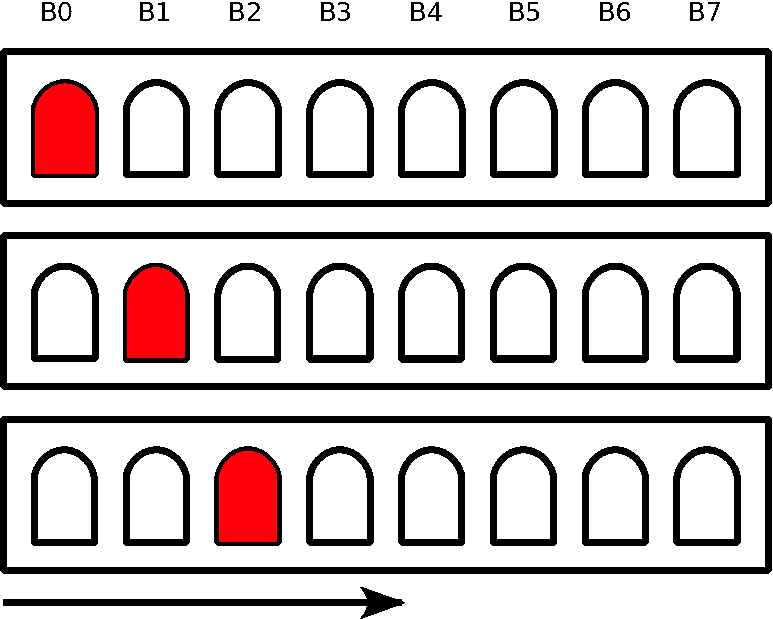
\includegraphics[scale=0.4]{diagrampdf-crop.pdf}
\end{center}
Écrire le code C correspondant sans utiliser la structure conditionnelle «~if~».


\ifnum\value{reponseCnt}=1
	\begin{uC}
	void SolutionA() {
		TRISB = 0xFF00;
		while(1)
		{
		  for (int i=0;i<7;i++)
		  {
		     LATB = (LATB & 0xFF00) | (0x0001 << i);
		     Delay_1ms(100);
		  }
		}
	}

	void SolutionB() {
		TRISB = 0xFF00;
		while(1)
		{
		  LATB = 0x0001;
		  for (int i=0;i<7;i++)
		  {
		     LATB = LATB << 1;
		     Delay_1ms(100);
		  }
		}
	}

	void SolutionC() {
		TRISB = 0xFF00;
		while(1)
		{
		  for (int i=0;i<7;i++)
		  {
		     LATB = 1 << i;
		     Delay_1ms(100);
		  }
		}
	}
\end{uC}
\fi

\end{Q}
\ifnum\value{reponseCnt}=1
  \newpage
\fi
\begin{Q}
	Un ouvre-porte $Z_1$ est commandé par deux boutons $a$ et $b$ qu'il faut actionner dans le bon ordre sous peine de déclencher une alarme $Z_2$.
	Celui-ci est décrit par la table de Huffman ci-dessous.
	Implémentez l'automate correspondant en C.

	\begin{center}
		\begin{tabular}{|l|l|l|l|l|l|l|} \hline
			\multirow{2}{*}{} & \multicolumn{4}{c|}{$ab$} & \multirow{2}{*}{$Z_1$} & \multirow{2}{*}{$Z_2$} \\ \cline{2-5}
			& 00 & 01 & 11 & 10 & & \\ \hline
			1 & \textbf{1} & 5 & 5 & 2 & 0 & 0 \\ \hline
			2 & 3 & 5 & 5 & \textbf{2} & 0 & 0 \\ \hline
			3 & \textbf{3} & 4 & 5 & 5 & 0 & 0 \\ \hline
			4 & 1 & \textbf{4} & 5 & 5 & 1 & 0 \\ \hline
			5 & 1 & \textbf{5} & \textbf{5} & \textbf{5} & 0 & 1 \\ \hline
		\end{tabular}
	\end{center}

\ifnum\value{reponseCnt}=1
  \lstinputlisting[language=c,%
	commentstyle=\color{colComments}\textit,%
	float=hbp,%
	basicstyle=\ttfamily\footnotesize, %
	identifierstyle=\color{colIdentifier}, %
	keywordstyle=\color{colKeys}, %
	stringstyle=\color{colString}, %
  otherkeywords={bool},%
	columns=flexible, %
	tabsize=2, %
	extendedchars=true, %
	showspaces=false, %
	showstringspaces=false, %
	% numbers=left, %
	numberstyle=\tiny, %
	breaklines=true, %
	breakautoindent=true, %
	captionpos=b,%
	frame=lines]{sm.c}
\fi

\end{Q}


%
% \begin{Q}
% 	L'approximation I(V) idéalisée avec seulement la tension de seuil est-elle une bonne approximation ?
% 	\label{Q:1}
% 	\reponse{Oui}%R
% \end{Q}


% \begin{figure}[H]
% 	\begin{center}
% 		\begin{circuitikz}\draw
% 			(0,0) node[anchor=east] {A} to [short,i>^=$I$] (1.5,0)
% 			(0,0) to [sDo, v=$V$] (2.5,0) node [anchor=west]{K}
% 		;\end{circuitikz}
% 	\end{center}
% \caption{Conventions électriques}
% \label{fig:zener_conv}
% \end{figure}

\end{document}
